The first step in integrating GPGPU-Sim into SST is to handle the interaction
with an SST CPU component. Since GPUs today function solely as co-processors,
functionally executing GPU-enabled binaries requires the CPU to initialize and
launch kernels of work to the GPU. In our model, the GPU is constructed out of
two discrete SST components -- a scheduler and a SM block \cite{v100}. When CUDA
functions are called from the CPU component, they are intercepted and translated
into messages that are sent over SST links to the GPU (along with the associated
parameters). Table \ref{tab:apis} enumerates the CUDA API calls currently intercepted
and sent to the GPU elements. These calls are enough to enable the execution of
a number of CUDA SDK kernels, DoE proxy apps as well as a collection of Kokkos Unit
tests. Table \ref{tab:kokkos_tests} lists the number of Kokkos unit tests that
pass with our current implementation of SST-GPU, which is about 60\%. There is
ongoing work with the PTX parser to increase the number of running kernels.


    \begin{table}[!htbp]
        \centering
        \setlength{\abovecaptionskip}{6pt plus 1pt minus 1pt}
        \captionsetup{width=.75\textwidth}
        \caption {Intercepted CUDA API Calls Forwarded to GPU Model}
            \begin{tabular}{|p{14cm} | p{3cm}|}
%             \multicolumn{1}{c} {\textbf{API Call}} \\
            \hline
            \texttt{\textunderscore \textunderscore cudaRegisterFatBinary} \\
            \hline
            \texttt{\textunderscore \textunderscore cudaRegisterFunction} \\
            \hline
            \texttt{cudaMalloc} \\
            \hline
            \texttt{cudaMemcpy} \\
            \hline
            \texttt{cudaConfigureCall} \\
            \hline
            \texttt{cudaSetupArgument} \\
            \hline
            \texttt{cudaFree} \\
            \hline
            \texttt{cudaLaunch} \\
            \hline
            \texttt{cudaGetLastError} \\
            \hline
            \texttt{\textunderscore \textunderscore cudaRegisterVar} \\
            \hline
            \texttt{cudaOccupancyMaxActiveBlocksPerMultiprocessorWithFlags} \\
            \hline
            \end{tabular}
        \label{tab:apis}
    \end{table}

      \begin{table}[!htbp]
         \centering
         \setlength{\abovecaptionskip}{6pt plus 1pt minus 1pt}
         \captionsetup{width=.75\textwidth}
         \caption {Functionally Passing Kokkos Unit Tests}
            \scalebox{0.56}{
            \tabcolsep=0.11cm\begin{tabular}{lll}
               \multicolumn{1}{c}{\textbf{Kernel Name}} & \multicolumn{1}{c}{\textbf{GPGPU-Sim}} & \multicolumn{1}{c}{\textbf{GPGPU-Sim/SST}} \\
               abs\_double & {\color[HTML]{32CB00} OK} & {\color[HTML]{32CB00} OK} \\
               abs\_mv\_double & {\color[HTML]{32CB00} OK} & {\color[HTML]{32CB00} OK} \\
               asum\_double & {\color[HTML]{32CB00} OK} & {\color[HTML]{32CB00} OK} \\
               axpby\_double & {\color[HTML]{32CB00} OK} & {\color[HTML]{32CB00} OK} \\
               axpby\_mv\_double & {\color[HTML]{32CB00} OK} & {\color[HTML]{32CB00} OK} \\
               axpy\_double & {\color[HTML]{32CB00} OK} & {\color[HTML]{32CB00} OK} \\
               axpy\_mv\_double & {\color[HTML]{32CB00} OK} & {\color[HTML]{32CB00} OK} \\
               dot\_double & {\color[HTML]{32CB00} OK} & {\color[HTML]{32CB00} OK} \\
               dot\_mv\_double & {\color[HTML]{32CB00} OK} & {\color[HTML]{32CB00} OK} \\
               mult\_double & {\color[HTML]{32CB00} OK} & {\color[HTML]{32CB00} OK} \\
               mult\_mv\_double & {\color[HTML]{32CB00} OK} & {\color[HTML]{32CB00} OK} \\
               nrm1\_double & {\color[HTML]{32CB00} OK} & {\color[HTML]{32CB00} OK} \\
               nrm1\_mv\_double & {\color[HTML]{32CB00} OK} & {\color[HTML]{32CB00} OK} \\
               nrm2\_double & {\color[HTML]{32CB00} OK} & {\color[HTML]{32CB00} OK} \\
               nrm2\_mv\_double & {\color[HTML]{32CB00} OK} & {\color[HTML]{32CB00} OK} \\
               nrm2\_squared\_double & {\color[HTML]{32CB00} OK} & {\color[HTML]{32CB00} OK} \\
               nrm2\_squared\_mv\_double & {\color[HTML]{32CB00} OK} & {\color[HTML]{32CB00} OK} \\
               nrminf\_double & {\color[HTML]{FE0000} FAILED} & {\color[HTML]{9B9B9B} PREVIOUS FAILED} \\
               nrminf\_mv\_double & {\color[HTML]{FE0000} FAILED} & {\color[HTML]{9B9B9B} PREVIOUS FAILED} \\
               reciprocal\_double & {\color[HTML]{FE0000} FAILED} & {\color[HTML]{9B9B9B} PREVIOUS FAILED} \\
               reciprocal\_mv\_double & {\color[HTML]{FE0000} FAILED} & {\color[HTML]{9B9B9B} PREVIOUS FAILED} \\
               scal\_double & {\color[HTML]{32CB00} OK} & {\color[HTML]{32CB00} OK} \\
               scal\_mv\_double & {\color[HTML]{32CB00} OK} & {\color[HTML]{32CB00} OK} \\
               sum\_double & {\color[HTML]{32CB00} OK} & {\color[HTML]{32CB00} OK} \\
               sum\_mv\_double & {\color[HTML]{32CB00} OK} & {\color[HTML]{32CB00} OK} \\
               update\_double & {\color[HTML]{32CB00} OK} & {\color[HTML]{32CB00} OK} \\
               update\_mv\_double & {\color[HTML]{32CB00} OK} & {\color[HTML]{32CB00} OK} \\
               gemv\_double & {\color[HTML]{FE0000} FAILED} & {\color[HTML]{9B9B9B} PREVIOUS FAILED} \\
               gemm\_double & {\color[HTML]{FE0000} FAILED} & {\color[HTML]{9B9B9B} PREVIOUS FAILED} \\
               sparse\_spgemm\_double\_int\_int\_TestExecSpace & {\color[HTML]{FE0000} FAILED} & {\color[HTML]{9B9B9B} PREVIOUS FAILED} \\
               sparse\_spadd\_double\_int\_int\_TestExecSpace & {\color[HTML]{FFC702} NOT PARSED} & {\color[HTML]{9B9B9B} PREVIOUS FAILED} \\
               sparse\_gauss\_seidel\_double\_int\_int\_TestExecSpace & {\color[HTML]{FFC702} NOT PARSED} & {\color[HTML]{9B9B9B} PREVIOUS FAILED} \\
               sparse\_block\_gauss\_seidel\_double\_int\_int\_TestExecSpace & {\color[HTML]{FFC702} NOT PARSED} & {\color[HTML]{9B9B9B} PREVIOUS FAILED} \\
               sparse\_crsmatrix\_double\_int\_int\_TestExecSpace & {\color[HTML]{FFC702} NOT PARSED} & {\color[HTML]{9B9B9B} PREVIOUS FAILED} \\
               sparse\_blkcrsmatrix\_double\_int\_int\_TestExecSpace & {\color[HTML]{FFC702} NOT PARSED} & {\color[HTML]{9B9B9B} PREVIOUS FAILED} \\
               sparse\_replaceSumIntoLonger\_double\_int\_int\_TestExecSpace & {\color[HTML]{FFC702} NOT PARSED} & {\color[HTML]{9B9B9B} PREVIOUS FAILED} \\
               sparse\_replaceSumInto\_double\_int\_int\_TestExecSpace & {\color[HTML]{FFC702} NOT PARSED} & {\color[HTML]{9B9B9B} PREVIOUS FAILED} \\
               sparse\_graph\_color\_double\_int\_int\_TestExecSpace & {\color[HTML]{FFC702} NOT PARSED} & {\color[HTML]{9B9B9B} PREVIOUS FAILED} \\
               sparse\_graph\_color\_d2\_double\_int\_int\_TestExecSpace & {\color[HTML]{FE0000} FAILED} & {\color[HTML]{9B9B9B} PREVIOUS FAILED} \\
               common\_ArithTraits & {\color[HTML]{FFC702} NOT PARSED} & {\color[HTML]{9B9B9B} PREVIOUS FAILED} \\
               common\_set\_bit\_count & {\color[HTML]{FE0000} FAILED} & {\color[HTML]{9B9B9B} PREVIOUS FAILED} \\
               common\_ffs & {\color[HTML]{32CB00} OK} & {\color[HTML]{32CB00} OK} \\
               batched\_scalar\_serial\_set\_double\_double & {\color[HTML]{32CB00} OK} & {\color[HTML]{FE0000} FAILED} \\
               batched\_scalar\_serial\_scale\_double\_double & {\color[HTML]{32CB00} OK} & {\color[HTML]{32CB00} OK} \\
               batched\_scalar\_serial\_gemm\_nt\_nt\_double\_double & {\color[HTML]{32CB00} OK} & {\color[HTML]{32CB00} OK} \\
               batched\_scalar\_serial\_gemm\_t\_nt\_double\_double & {\color[HTML]{32CB00} OK} & {\color[HTML]{32CB00} OK} \\
               batched\_scalar\_serial\_gemm\_nt\_t\_double\_double & {\color[HTML]{32CB00} OK} & {\color[HTML]{32CB00} OK} \\
               batched\_scalar\_serial\_gemm\_t\_t\_double\_double & {\color[HTML]{32CB00} OK} & {\color[HTML]{32CB00} OK} \\
               batched\_scalar\_serial\_trsm\_l\_l\_nt\_u\_double\_double & {\color[HTML]{32CB00} OK} & {\color[HTML]{32CB00} OK} \\
               batched\_scalar\_serial\_trsm\_l\_l\_nt\_n\_double\_double & {\color[HTML]{FE0000} FAILED} & {\color[HTML]{9B9B9B} PREVIOUS FAILED} \\
               batched\_scalar\_serial\_trsm\_l\_u\_nt\_u\_double\_double & {\color[HTML]{32CB00} OK} & {\color[HTML]{32CB00} OK} \\
               batched\_scalar\_serial\_trsm\_l\_u\_nt\_n\_double\_double & {\color[HTML]{FE0000} FAILED} & {\color[HTML]{9B9B9B} PREVIOUS FAILED} \\
               batched\_scalar\_serial\_trsm\_r\_u\_nt\_u\_double\_double & {\color[HTML]{32CB00} OK} & {\color[HTML]{32CB00} OK} \\
               batched\_scalar\_serial\_trsm\_r\_u\_nt\_n\_double\_double & {\color[HTML]{FE0000} FAILED} & {\color[HTML]{9B9B9B} PREVIOUS FAILED} \\
               batched\_scalar\_serial\_lu\_double & {\color[HTML]{32CB00} OK} & {\color[HTML]{FE0000} FAILED} \\
               batched\_scalar\_serial\_gemv\_nt\_double\_double & {\color[HTML]{32CB00} OK} & {\color[HTML]{32CB00} OK} \\
               batched\_scalar\_serial\_gemv\_t\_double\_double & {\color[HTML]{32CB00} OK} & {\color[HTML]{32CB00} OK} \\
               batched\_scalar\_serial\_trsv\_l\_nt\_u\_double\_double & {\color[HTML]{32CB00} OK} & {\color[HTML]{FE0000} FAILED} \\
               batched\_scalar\_serial\_trsv\_l\_nt\_n\_double\_double & {\color[HTML]{FE0000} FAILED} & {\color[HTML]{9B9B9B} PREVIOUS FAILED} \\
               batched\_scalar\_serial\_trsv\_u\_nt\_u\_double\_double & {\color[HTML]{32CB00} OK} & {\color[HTML]{FE0000} FAILED} \\
               batched\_scalar\_serial\_trsv\_u\_nt\_n\_double\_double & {\color[HTML]{FE0000} FAILED} & {\color[HTML]{9B9B9B} PREVIOUS FAILED} \\
               batched\_scalar\_team\_set\_double\_double & {\color[HTML]{32CB00} OK} & {\color[HTML]{FE0000} FAILED} \\
               batched\_scalar\_team\_scale\_double\_double & {\color[HTML]{32CB00} OK} & {\color[HTML]{32CB00} OK} \\
               batched\_scalar\_team\_gemm\_nt\_nt\_double\_double & {\color[HTML]{32CB00} OK} & {\color[HTML]{32CB00} OK} \\
               batched\_scalar\_team\_gemm\_t\_nt\_double\_double & {\color[HTML]{32CB00} OK} & {\color[HTML]{32CB00} OK} \\
               batched\_scalar\_team\_gemm\_nt\_t\_double\_double & {\color[HTML]{32CB00} OK} & {\color[HTML]{32CB00} OK} \\
               batched\_scalar\_team\_gemm\_t\_t\_double\_double & {\color[HTML]{32CB00} OK} & {\color[HTML]{32CB00} OK} \\
               batched\_scalar\_team\_trsm\_l\_l\_nt\_u\_double\_double & {\color[HTML]{32CB00} OK} & {\color[HTML]{32CB00} OK} \\
               batched\_scalar\_team\_trsm\_l\_l\_nt\_n\_double\_double & {\color[HTML]{FE0000} FAILED} & {\color[HTML]{9B9B9B} PREVIOUS FAILED} \\
               batched\_scalar\_team\_trsm\_l\_u\_nt\_u\_double\_double & {\color[HTML]{32CB00} OK} & {\color[HTML]{32CB00} OK} \\
               batched\_scalar\_team\_trsm\_l\_u\_nt\_n\_double\_double & {\color[HTML]{FE0000} FAILED} & {\color[HTML]{9B9B9B} PREVIOUS FAILED} \\
               batched\_scalar\_team\_trsm\_r\_u\_nt\_u\_double\_double & {\color[HTML]{32CB00} OK} & {\color[HTML]{32CB00} OK} \\
               batched\_scalar\_team\_trsm\_r\_u\_nt\_n\_double\_double & {\color[HTML]{FE0000} FAILED} & {\color[HTML]{9B9B9B} PREVIOUS FAILED} \\
               batched\_scalar\_team\_lu\_double & {\color[HTML]{32CB00} OK} & {\color[HTML]{FE0000} FAILED} \\
               batched\_scalar\_team\_gemv\_nt\_double\_double & {\color[HTML]{32CB00} OK} & {\color[HTML]{32CB00} OK} \\
               batched\_scalar\_team\_gemv\_t\_double\_double & {\color[HTML]{32CB00} OK} & {\color[HTML]{32CB00} OK}
            \end{tabular} }
         \label{tab:kokkos_tests}
      \end{table}


Aside from the basic functional model provided by GPU-SST, an initial
performance model has also been developed. Figure \ref{fig:gpu_sched} details
the overall architecture. A CPU component (Ariel in the initial implementation)
is connected via SST links to 2 GPU components: the SMs, which implement the
timing and functional model for the GPU cores, and a centralized kernel and CTA
scheduler (GPUSched). When CUDA calls are intercepted from the CPU, messages are
sent to both the SMs and the GPU scheduler. Messages related to memory copies
and other information necessary to populate the GPU functional model are sent
directly to the SMs element, since the functional model for executing the GPU
kernels lives inside the SMs element. Calls related to enqueuing kernels for
execution are sent to the GPU scheduler element, which co-ordinates the
launching of CTAs on the SMs, e.g. \texttt{cudaConfigureCall} and
\texttt{cudaLaunch}.


   \begin{figure}[!htb]
      \centering
      \setlength{\abovecaptionskip}{6pt plus 1pt minus 1pt}
      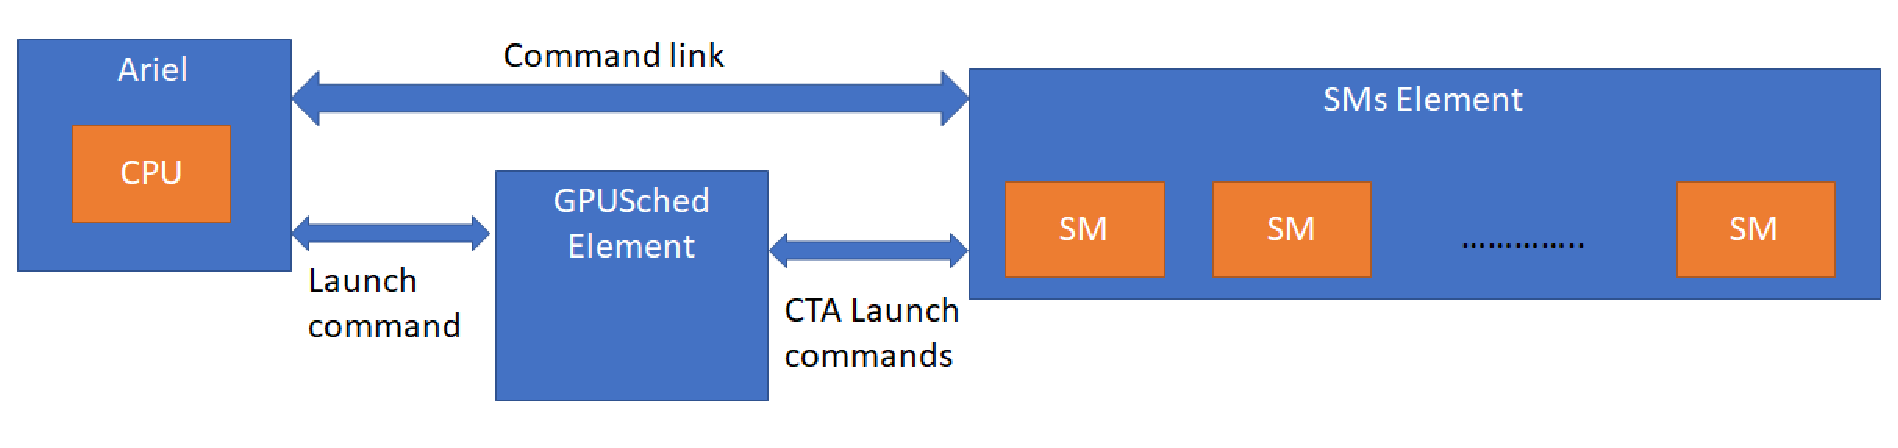
\includegraphics[width=.90\textwidth,keepaspectratio]{figures/2_1.eps}
      \captionsetup{width=.90\textwidth}
      \caption{SST Element architecture for kernel/CTA scheduler and SMs components}
      \label{fig:gpu_sched}
   \end{figure}


As CTAs complete on the SMs, messages are sent back to the GPU scheduler
element, which pushes new work to the SMs from enqueued kernels as needed.
Memory copies from the CPU to GPU address space are handled on a configurable
page-size granularity, similar to how conventional CUDA unified memory handles
the transfer of data from CPU to GPU memories.

   \begin{figure}[!htb]
      \centering
      \setlength{\abovecaptionskip}{6pt plus 1pt minus 1pt}
      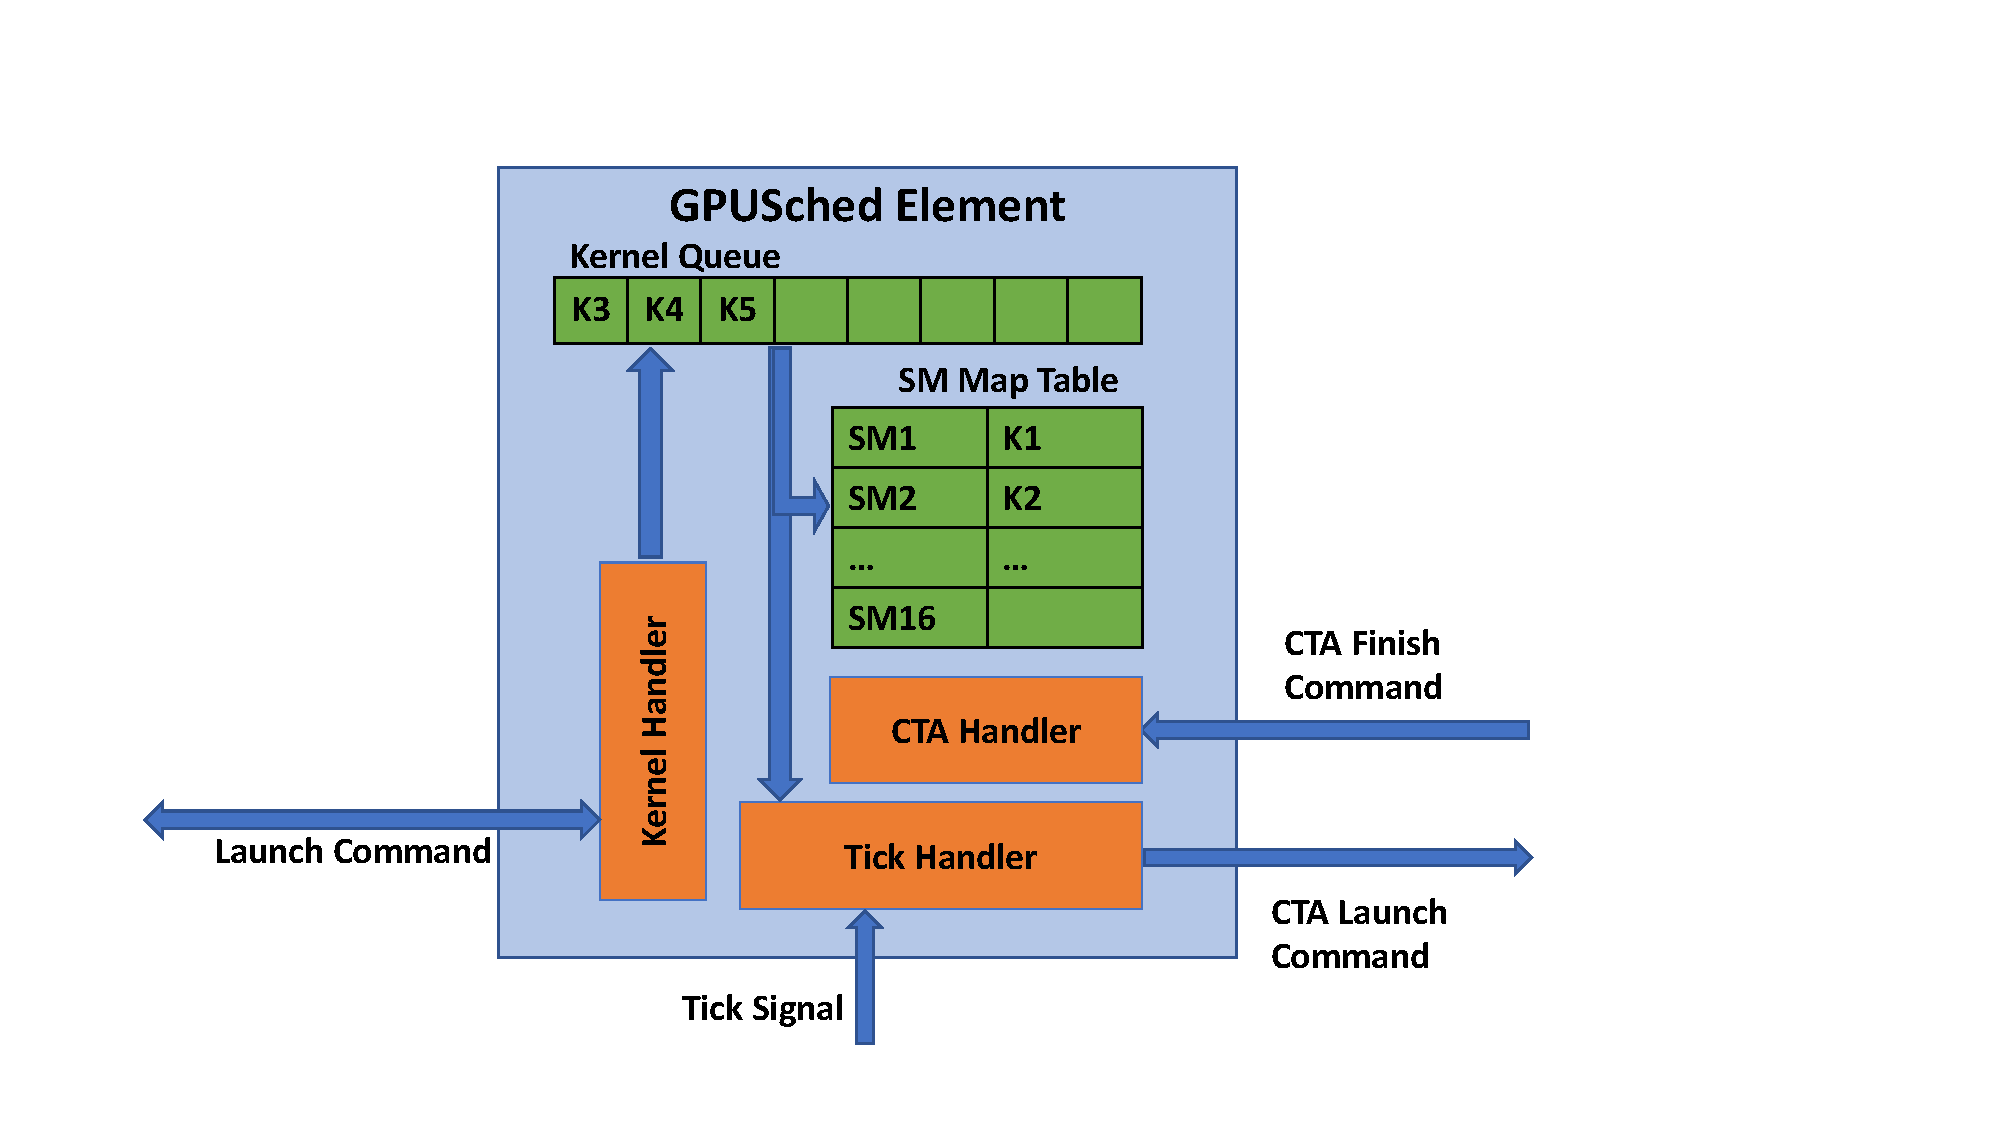
\includegraphics[width=.90\textwidth,keepaspectratio]{figures/scheduler.pdf}
      \captionsetup{width=.75\textwidth}
      \caption{Centralized GPU Scheduler component}
      \label{fig:sched}
   \end{figure}

The centralized GPU scheduler receives kernel launch commands from the CPU, then
issues CTA launch commands to the SMs. The scheduler also receives notifications
from the SMs when the CTAs finish. The reception of kernel launch and CTA
complete notifications are independent, therefore we designed a different
handler for each type of message. Figure~\ref{fig:sched} shows the design of the
centralized kernel and CTA Scheduler. The kernel handler listens to calls from a
CPU component and pushes kernel launch information to the kernel queue when it
receives kernel configure and launch commands. The SM map table contains CTA
slots for each of the SMs, which is reserved when launching a CTA and released when a
message indicating that a CTA has finished is received from the SMs. The
scheduler clock ticks trigger CTA launches to SMs, when space is available and
there is a pending kernel. On every tick, the scheduler issues a CTA launch
command for currently unfinished kernels if any CTA slot is available or tries
to fetch a new kernel launch from kernel queue. The CTA handler also waits for
SMs to reply the CTA finish message, so that CTA slots in the SM map table may
be freed.
